\documentclass[11pt,a4paper]{article}
\usepackage[utf8]{inputenc}
\usepackage[spanish]{babel}
\usepackage{amsmath}
\usepackage{amsfonts}
\usepackage{amssymb}
\usepackage{graphicx}
\usepackage[left=2cm,right=2cm,top=2cm,bottom=2cm]{geometry}
\title{Universidad Politécnica de la Zona Metropolitana de Guadalajara}
\begin{document}

\maketitle


\begin{figure}[hbtp]
\begin{center}

\includegraphics[scale=1]{1.jpeg}
\end{center}
\end{figure}


\begin{center}
\author{Sistemas Electrónicos de Interfaz\\
Barrera Vazquez Omar\\
Ing. Mecatrónica 4B}
\end{center}

\newpage

\section{Arreglos de amplificadores tipo B}

Un arreglo de tipo B es parecido a un arreglo tipo A pero tiene un mejora en cuanto el rendimiento. En los arreglos tipo A se observan deficiencias al momento de amplificar una señal, en cambio en el arreglo tipo B es diferente la amplificación de una intensidad como a continuación se explica el funcionamiento de un arreglo tipo \emph{push pull}. 

\subsection{Funcionamiento de amplificador tipo B}

un amplificador tipo B utiliza dos transistores en contrafase de manera tal que están denominados como \emph{Q1} y \emph{Q2} por lo que al considerar una alimentación de corriente alterna, cada transistor trabajara con la mitad del ciclo. el denominado \textbf{Q1} trabajara con un semiciclo tomando la parte positiva del ciclo de tension y lo amplificara, esto ayudara a eliminar en la medida de lo posible la distorsión al ser amplificado. Mientras Q1 hace el devanado del primer semiciclo el otro transistor deja de funcionar, pero cuando Q1 termina \textbf{Q2} comienza a trabajar con el semiciclo negativo, lo amplifica y manda la señal al emisor, de este modo se completa se ciclo de circulación de la corriente alterna en un arreglo tipo B 


\section{Analizando funcionamiento en amplificador tipo B}

Se analizara un amplificador de audio de tipo B en el cual participa dos transistores de potencia, un transformador y un altavoz, se muestra a continuacion en la figura 1: \cite{malvino1991principios}

\begin{figure}[h]
\begin{center}
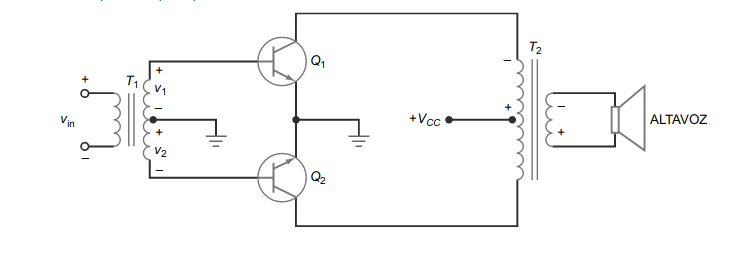
\includegraphics[scale=0.7]{2.png}
\caption{arreglo de amplificador tipo B}
\end{center}
\end{figure}

El funcionamiento que se realiza en la imagen anterior es una muestra de dos transistores en contrafase que al trabajar cada uno amplifica un semiciclo de manera tal que trabajando los dos se amplifica la señal del altavoz sin tener en cuenta tanta distorsión. Tal es el funcionamiento del \emph{arreglo tipo B} que su rendimiento es de 78,6 respecto a 100, comparándolo con el arreglo tipo A es triple eficiencia.

No todo tiene su perfección, el cuestiona miento es el uso de un transformador para la entrega de voltaje en los transistores, normalmente son grandes y poco usados en la actualidad, estos se han ido reemplazando por otro tipo de circuitos con mejorías.

Cabe destacar que los amplificadores de tipo B la mitad del ciclo que no están recibiendo una señal, evitan el uso de gasto de potencia, por lo que eso lo refleja en su rendimiento.

\newpage

\section{Recta de carga en continua}

En circuitos de arreglo tipo B segun la configuracion puesta si es \emph{npn} o \emph{pnp} en un seguidor de emisor, tomara una complicacion en la recta de carga de lo transistores, puesto que no hay una resistencia en continua su recta sera de manera vertical, lo que ocasionara un peligro de inestabilidad en el punto de corte, esto puede ser causado por distintos factores ajenos al circuito como la temperatura. Como se observa en la figura 2: \cite{malvino1991principios}

\begin{figure}[h]
\begin{center}
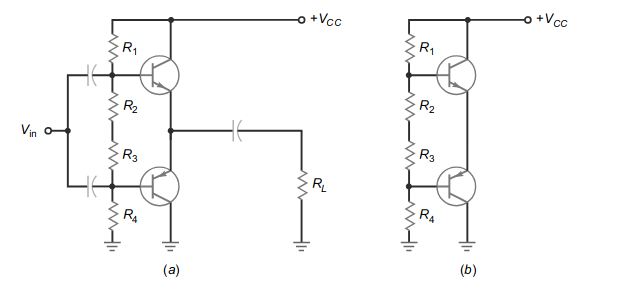
\includegraphics[scale=0.7]{3.png}
\end{center}
\end{figure}

\subsection{Recta de carga en alterna}

Esta parte de la recta de la carga en alterna dicta la parte de la tension en un transistor en cual en un semiciclo de conducción puede variar entre la saturación y punto de corte el cual esta denostado en la siguiente ecuación:

\begin{center}
\begin{equation}
MPP=Vcc
\end{equation}
\end{center}

\section{Distorsión de cruce}

En el momento de la conduccion en cualquiera de los dos transistores, al existir una conduccion a travez de ellos y no tener una polarizacion en sus diodos emisores, esto provocara que en la salida de tension en alterna tenga una ligera distorsion por lo que podria provocarnos una mala señal de salida, para solucionar esta parte es necesario polarizar los diodos, lo que provocara que la barrera de conducion del diodo del transistor sea alrededor de los 0,7 volts, esto implicara tanto para el semiciclo positivo como para el negativo. Parte de un ejemplo lo podemo ver en la figura 3:\cite{malvino1991principios}

\begin{figure}[h]
 \begin{center}
 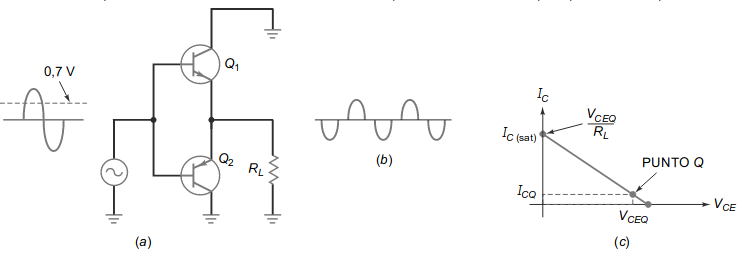
\includegraphics[scale=0.35]{4.png}
 \caption{demostración de salida polarizada y no polarizada}
 \end{center}
\end{figure}

\newpage

\bibliographystyle{apalike} 
\bibliography{ref}















\end{document}